
\documentclass[conference]{IEEEtran}
\IEEEoverridecommandlockouts

% -------------------- PACKAGES --------------------
\usepackage[T1]{fontenc}
\usepackage{cite}
\usepackage{url}
\usepackage{graphicx}
\usepackage{booktabs}
\usepackage{tabularx}
\usepackage{array}
\usepackage{enumitem}
\usepackage{tikz}
\usetikzlibrary{arrows.meta,positioning,shapes.geometric,calc}
\usepackage{balance}
\usepackage{microtype}

\setlist{nosep,leftmargin=*}
\renewcommand{\arraystretch}{1.12}
\newcolumntype{Y}{>{\raggedright\arraybackslash}X}

% -------------------- TITLE --------------------
\title{Software Architecture Document for the Electronics Store Inventory Management System (SEIMS)}

% -------------------- AUTHORS --------------------
\author{
\IEEEauthorblockN{Karthik Peddibhotla}
\IEEEauthorblockA{
\textit{Department of Computer Science \& Engineering}\\
PES University\\
SRN: PES2UG24CS348\\
karthikpeddibhotla5@gmail.com
}
\and
\IEEEauthorblockN{Paridhi Bajpai}
\IEEEauthorblockA{
\textit{Department of Computer Science \& Engineering}\\
PES University\\
SRN: PES2UG24CS337\\
paridhi.bajaj03@gmail.com
}
\and
\IEEEauthorblockN{Niharika S Murthy}
\IEEEauthorblockA{
\textit{Department of Computer Science \& Engineering}\\
PES University\\
SRN: PES2UG24CS316\\
niharika.sm0@gmail.com
}
\and
\IEEEauthorblockN{P. Dhanush}
\IEEEauthorblockA{
\textit{Department of Computer Science \& Engineering}\\
PES University\\
SRN: PES2UG24CS333\\
penchalpaadudhanush@gmail.com
}
}

\begin{document}

\maketitle

% -------------------- ABSTRACT --------------------
\begin{abstract}
This Software Architecture Document (SAD) describes the architecture of the Electronics Store Inventory Management System (SEIMS). It presents the system organization, technology stack, major software components, database structure, request workflows, security considerations, API design, testing organization, and deployment approach. The system uses a Flask-based web application with an SQLite relational database and server-rendered HTML views. The architecture separates presentation, application processing, and data persistence to support maintainability, reliability, and testability.
\end{abstract}

\begin{IEEEkeywords}
Software Architecture Document, SEIMS, three-layer architecture, Flask, SQLite, component design, security, inventory management.
\end{IEEEkeywords}

% ==================================================
\section{Introduction}
% ==================================================

\subsection{Purpose}
This Software Architecture Document describes the high-level design of the Electronics Store Inventory Management System. It explains the system's major structures, architectural decisions, component responsibilities, database organization, workflows, interfaces, and security mechanisms. It complements the Software Requirements Specification (SRS) and provides a technical reference for development, testing, and maintenance.

\subsection{Scope}
The architecture covers Flask request handling, server-side template rendering, SQLite database access, authentication and session handling, inventory operations, stock classification, reporting, CSV export, automated testing, and the intended deployment model.

\subsection{Definitions and Acronyms}

\begin{table}[!t]
\caption{Architectural Acronyms}
\label{tab:acronyms}
\centering
\small
\begin{tabularx}{\columnwidth}{lY}
\toprule
\textbf{Term} & \textbf{Meaning}\\
\midrule
SAD & Software Architecture Document\\
SRS & Software Requirements Specification\\
MVC & Model-View-Controller pattern\\
WSGI & Web Server Gateway Interface\\
SKU & Stock Keeping Unit\\
CRUD & Create, Read, Update, Delete\\
API & Application Programming Interface\\
\bottomrule
\end{tabularx}
\end{table}

\subsection{Document Organization}
The remainder of this document describes the architectural overview, component design, database architecture, detailed workflows, API design, security architecture, testing, deployment, quality attributes, risks, and references.

% ==================================================
\section{Architectural Overview}
% ==================================================

\subsection{System Overview}
SEIMS follows a three-layer web architecture. The presentation layer renders browser-facing pages using HTML, CSS, and Jinja2 templates. The application layer uses Python and Flask to handle routes, sessions, validation, and business rules. The data layer uses SQLite to persist user and component records.

The browser communicates with the Flask application through HTTP requests. Flask processes requests, interacts with the database, and returns rendered HTML pages or downloadable CSV responses.

\begin{figure}[!t]
\centering
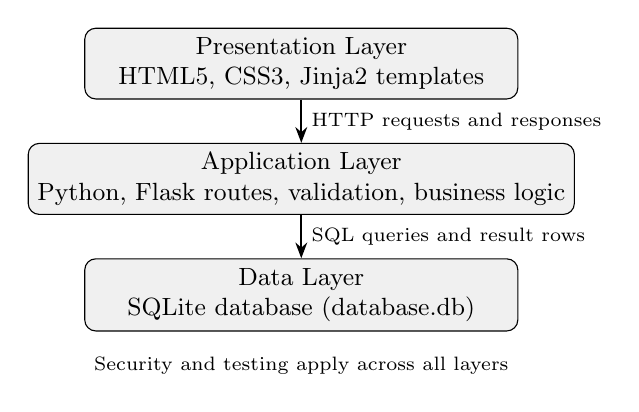
\begin{tikzpicture}[
layer/.style={
draw,rounded corners,align=center,
minimum width=5.5cm,minimum height=0.85cm,
font=\small
},
arr/.style={-{Stealth[length=2mm]},thick}
]
\node[layer,fill=gray!12] (pres)
{Presentation Layer\\HTML5, CSS3, Jinja2 templates};

\node[layer,fill=gray!12,below=0.55cm of pres] (app)
{Application Layer\\Python, Flask routes, validation, business logic};

\node[layer,fill=gray!12,below=0.55cm of app] (data)
{Data Layer\\SQLite database (database.db)};

\draw[arr] (pres)--node[right,font=\scriptsize]
{HTTP requests and responses}(app);

\draw[arr] (app)--node[right,font=\scriptsize]
{SQL queries and result rows}(data);

\node[font=\scriptsize,align=center,below=0.2cm of data]
{Security and testing apply across all layers};
\end{tikzpicture}
\caption{Three-Layer Architecture of SEIMS}
\label{fig:architecture}
\end{figure}

\subsection{Architectural Pattern}
The system uses a layered architectural pattern with responsibilities separated into presentation, application, and data layers. Flask routes coordinate request processing and application logic, HTML templates provide the user interface, and SQLite manages persistent records.

The design also follows selected Model-View-Controller principles:
\begin{itemize}
\item \textbf{Model:} Inventory and user data stored in SQLite.
\item \textbf{View:} HTML templates rendered using Jinja2.
\item \textbf{Controller:} Flask routes and request handlers.
\end{itemize}

\subsection{Architectural Goals}
The architecture is guided by the following goals:
\begin{itemize}
\item \textbf{Simplicity and maintainability:} Separate templates, styles, backend routing, and database operations.
\item \textbf{Data integrity:} Apply database constraints for unique SKUs and valid stock and price values.
\item \textbf{Security baseline:} Use password hashing and authenticated-session checks for protected routes.
\item \textbf{Testability:} Verify application behavior through automated tests.
\item \textbf{Usability:} Provide clear inventory views, dashboard summaries, filters, and reports.
\end{itemize}

\subsection{Technology Stack}

\begin{table}[!t]
\caption{Technology Stack Mapping}
\label{tab:stack}
\centering
\small
\begin{tabularx}{\columnwidth}{l l Y}
\toprule
\textbf{Area} & \textbf{Technology} & \textbf{Responsibility}\\
\midrule
Presentation & HTML, CSS, Jinja2 & User interface rendering\\
Application & Python, Flask & Routing and business logic\\
Database & SQLite 3 & Relational data persistence\\
Security & Werkzeug & Password hashing utilities\\
Testing & Pytest & Automated verification\\
Version Control & Git, GitHub & Source control and collaboration\\
CI & GitHub Actions & Automated test workflow\\
\bottomrule
\end{tabularx}
\end{table}

% ==================================================
\section{Component Design}
% ==================================================

\subsection{Component Breakdown}
The application is organized around the following functional components:

\begin{itemize}
\item \textbf{Authentication Component:} Verifies credentials and manages the user session.
\item \textbf{Dashboard Component:} Retrieves and displays inventory summary counts.
\item \textbf{Inventory Display Component:} Presents component records and supports search and filtering.
\item \textbf{Inventory Management Component:} Creates, reads, updates, and deletes component records.
\item \textbf{Stock Classifier:} Determines component status using quantity and minimum stock level.
\item \textbf{Availability Reporter:} Groups inventory records by stock status.
\item \textbf{CSV Exporter:} Produces downloadable CSV inventory data.
\item \textbf{Database Handler:} Manages SQLite connections and database queries.
\end{itemize}

\subsection{Component Interaction}
Fig.~\ref{fig:components} shows the logical relationships between the functional components, Flask application, and SQLite database. These components represent logical responsibilities and may be implemented within the main Flask application module.

\begin{figure}[!t]
\centering
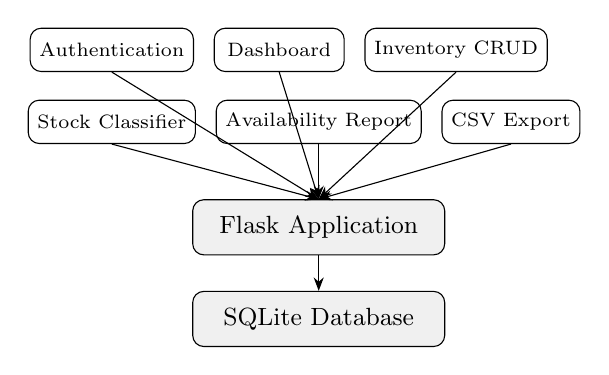
\begin{tikzpicture}[
c/.style={
draw,rounded corners,align=center,
minimum width=1.65cm,minimum height=0.55cm,
font=\scriptsize
},
core/.style={
draw,rounded corners,fill=gray!12,
align=center,minimum width=3.2cm,
minimum height=0.7cm,font=\small
},
arr/.style={-{Stealth[length=1.7mm]},thin}
]
\node[c] (auth) {Authentication};
\node[c,right=0.25cm of auth] (dash) {Dashboard};
\node[c,right=0.25cm of dash] (crud) {Inventory CRUD};

\node[c,below=0.35cm of auth] (class) {Stock Classifier};
\node[c,right=0.25cm of class] (report) {Availability Report};
\node[c,right=0.25cm of report] (csv) {CSV Export};

\node[core,below=0.7cm of report] (flask)
{Flask Application};

\node[core,below=0.45cm of flask] (db)
{SQLite Database};

\draw[arr] (auth.south)--(flask.north);
\draw[arr] (dash.south)--(flask.north);
\draw[arr] (crud.south)--(flask.north);
\draw[arr] (class.south)--(flask.north);
\draw[arr] (report.south)--(flask.north);
\draw[arr] (csv.south)--(flask.north);
\draw[arr] (flask)--(db);
\end{tikzpicture}
\caption{Logical Component Architecture}
\label{fig:components}
\end{figure}

\subsection{Component Responsibilities}
The authentication component verifies user credentials before allowing access to protected functions. Inventory management handles component creation, modification, deletion, and retrieval. The stock classifier evaluates component quantities against configured minimum stock levels. The reporting component groups components by status, while the CSV exporter prepares inventory information for download.

% ==================================================
\section{Database Architecture}
% ==================================================

\subsection{Data Model}
The database stores user credentials as password hashes and component inventory details. The Users table stores account information. The Components table stores identifying information, category, quantity, price, and minimum stock level.

\begin{figure}[!t]
\centering
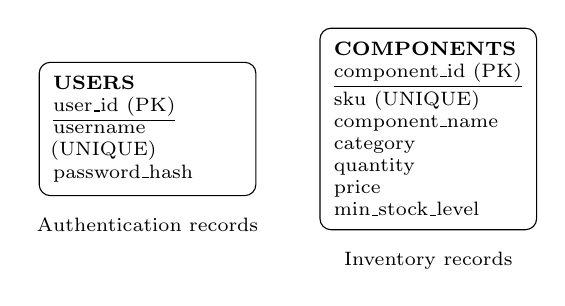
\begin{tikzpicture}[
entity/.style={
draw,rounded corners,align=left,
font=\scriptsize,inner sep=5pt,
text width=2.4cm
}
]
\node[entity] (users) {
\textbf{USERS}\\
\underline{user\_id (PK)}\\
username (UNIQUE)\\
password\_hash
};

\node[entity,right=0.8cm of users] (components) {
\textbf{COMPONENTS}\\
\underline{component\_id (PK)}\\
sku (UNIQUE)\\
component\_name\\
category\\
quantity\\
price\\
min\_stock\_level
};

\node[below=0.15cm of users,font=\scriptsize]
{Authentication records};

\node[below=0.15cm of components,font=\scriptsize]
{Inventory records};
\end{tikzpicture}
\caption{Logical Database Entities}
\label{fig:erd}
\end{figure}

\subsection{Components Table Schema}

\begin{table}[!t]
\caption{Components Table Schema}
\label{tab:components}
\centering
\small
\begin{tabularx}{\columnwidth}{l l Y}
\toprule
\textbf{Column} & \textbf{Type} & \textbf{Constraint}\\
\midrule
component\_id & INTEGER & Primary key, auto-increment\\
sku & TEXT & Unique identifier\\
component\_name & TEXT & Required component name\\
category & TEXT & Required category\\
quantity & INTEGER & Non-negative value\\
price & REAL & Non-negative value\\
min\_stock\_level & INTEGER & Default 10, non-negative\\
\bottomrule
\end{tabularx}
\end{table}

\subsection{Users Table Schema}

\begin{table}[!t]
\caption{Users Table Schema}
\label{tab:users}
\centering
\small
\begin{tabularx}{\columnwidth}{l l Y}
\toprule
\textbf{Column} & \textbf{Type} & \textbf{Constraint}\\
\midrule
user\_id & INTEGER & Primary key, auto-increment\\
username & TEXT & Required and unique\\
password\_hash & TEXT & Required password hash\\
\bottomrule
\end{tabularx}
\end{table}

\subsection{Data Integrity}
The database design uses primary keys to identify records and uniqueness constraints to prevent duplicate usernames and SKUs. Quantity, price, and minimum stock level are expected to be non-negative. Application-level validation and database constraints work together to maintain data integrity.

% ==================================================
\section{Detailed Design and Workflows}
% ==================================================

\subsection{Authentication Workflow}
The authentication workflow begins when a user submits login credentials through the browser. Flask receives the request, retrieves the matching user record from SQLite, verifies the submitted password against the stored password hash, and establishes an authenticated session when verification succeeds. If credentials are invalid, the application returns an authentication failure response.

\begin{figure}[!t]
\centering
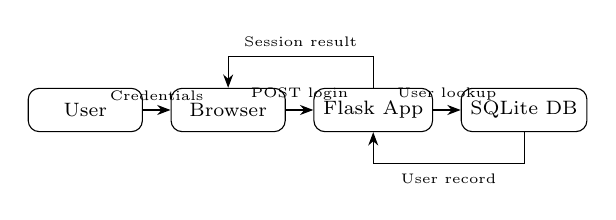
\begin{tikzpicture}[
p/.style={
draw,rounded corners,align=center,
minimum width=1.45cm,minimum height=0.55cm,
font=\scriptsize
},
arr/.style={-{Stealth[length=1.7mm]},thin}
]
\node[p] (u) {User};
\node[p,right=0.35cm of u] (b) {Browser};
\node[p,right=0.35cm of b] (f) {Flask App};
\node[p,right=0.35cm of f] (d) {SQLite DB};

\draw[arr] (u)--node[above,font=\tiny]{Credentials}(b);
\draw[arr] (b)--node[above,font=\tiny]{POST login}(f);
\draw[arr] (f)--node[above,font=\tiny]{User lookup}(d);

\draw[arr] (d.south) -- ++(0,-0.4) -|
node[below,pos=0.25,font=\tiny]{User record}(f.south);

\draw[arr] (f.north) -- ++(0,0.4) -|
node[above,pos=0.25,font=\tiny]{Session result}(b.north);
\end{tikzpicture}
\caption{Authentication Request Workflow}
\label{fig:authworkflow}
\end{figure}

\subsection{Inventory Update Workflow}
For an inventory update, the authenticated user submits revised component information. Flask validates the input and performs a parameterized database update. The application then returns an updated page or an appropriate validation message. Database constraints provide additional protection for values such as SKU uniqueness and non-negative quantity and price.

\begin{figure}[!t]
\centering
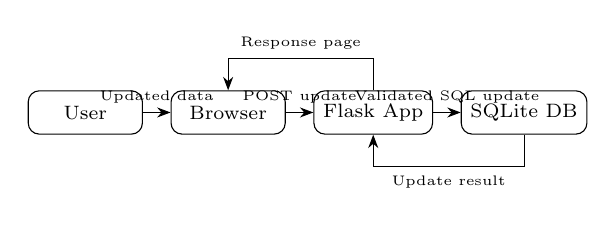
\begin{tikzpicture}[
p/.style={
draw,rounded corners,align=center,
minimum width=1.45cm,minimum height=0.55cm,
font=\scriptsize
},
arr/.style={-{Stealth[length=1.7mm]},thin}
]
\node[p] (user) {User};
\node[p,right=0.35cm of user] (browser) {Browser};
\node[p,right=0.35cm of browser] (flask) {Flask App};
\node[p,right=0.35cm of flask] (db) {SQLite DB};

\draw[arr] (user)--node[above,font=\tiny]{Updated data}(browser);
\draw[arr] (browser)--node[above,font=\tiny]{POST update}(flask);
\draw[arr] (flask)--node[above,font=\tiny]{Validated SQL update}(db);

\draw[arr] (db.south) -- ++(0,-0.4) -|
node[below,pos=0.25,font=\tiny]{Update result}(flask.south);

\draw[arr] (flask.north) -- ++(0,0.4) -|
node[above,pos=0.25,font=\tiny]{Response page}(browser.north);
\end{tikzpicture}
\caption{Inventory Update Workflow}
\label{fig:updateworkflow}
\end{figure}

% ==================================================
\section{API and Interface Design}
% ==================================================

\subsection{Browser Interface}
The browser interface provides pages for authentication, dashboard summaries, inventory display, component creation, component editing, and availability reporting. Templates are rendered by Flask using Jinja2.

\subsection{Application Interfaces}
The Flask application exposes browser-facing routes for user authentication, inventory operations, dashboard information, reports, and CSV export. The exact route names and HTTP methods are determined by the implemented application.

\begin{table}[!t]
\caption{Logical Application Interface Design}
\label{tab:api}
\centering
\small
\begin{tabularx}{\columnwidth}{l l Y}
\toprule
\textbf{Operation} & \textbf{Method} & \textbf{Purpose}\\
\midrule
Login & GET/POST & Display login and process credentials\\
Logout & GET/POST & End the authenticated session\\
Dashboard & GET & Display inventory summaries\\
Inventory & GET & Display and filter components\\
Add component & GET/POST & Display form and create a record\\
Edit component & GET/POST & Display form and update a record\\
Delete component & POST & Delete a selected record\\
Availability report & GET & Display stock classifications\\
CSV export & GET & Download inventory data\\
\bottomrule
\end{tabularx}
\end{table}

The table describes logical application operations. Actual route paths and methods should be checked against the current Flask implementation before submission.

\subsection{Communication Interface}
The browser communicates with the Flask application through HTTP requests and responses. The local development environment uses the configured Flask development port. A production deployment should use HTTPS.

% ==================================================
\section{Error Handling}
% ==================================================

The application should handle errors in a controlled manner to prevent invalid operations and provide understandable feedback.

\begin{itemize}
\item \textbf{Authentication errors:} Invalid credentials should result in an authentication failure message.
\item \textbf{Validation errors:} Missing or invalid component values should be rejected with appropriate feedback.
\item \textbf{Database errors:} Database operation failures should be handled without exposing internal database details to users.
\item \textbf{Missing records:} Requests for unavailable component records should return an appropriate not-found response or message.
\item \textbf{Access errors:} Unauthenticated users should be redirected to the login page or denied access to protected operations.
\end{itemize}

% ==================================================
\section{Security Architecture}
% ==================================================

The security architecture addresses confidentiality, integrity, and controlled access to inventory functions.

\begin{itemize}
\item \textbf{Password protection:} Passwords are stored using Werkzeug password-hashing utilities rather than plaintext passwords.
\item \textbf{Session guarding:} Protected endpoints use the application's authentication and session checks.
\item \textbf{SQL injection defence:} Database operations should use parameterized SQLite queries rather than directly concatenating untrusted input into SQL statements.
\item \textbf{Input constraints:} Application validation and database constraints reject invalid values, including negative quantities and duplicate SKUs.
\item \textbf{Secret management:} Production deployment should use a securely generated secret key supplied through environment configuration.
\item \textbf{Transport security:} HTTPS should be configured for production deployment to protect credentials and session traffic in transit.
\end{itemize}

The production secret-key and HTTPS requirements describe deployment expectations and should not be interpreted as completed deployment features unless they have been configured and verified.

% ==================================================
\section{Testing Architecture}
% ==================================================

The project uses Pytest to automate verification of application behavior. The test organization described in the project materials is summarized in Table~\ref{tab:tests}.

\begin{table}[!t]
\caption{Automated Test Suite Structure}
\label{tab:tests}
\centering
\small
\begin{tabularx}{\columnwidth}{lY}
\toprule
\textbf{Test File} & \textbf{Focus Area}\\
\midrule
test\_app.py & Routes, sessions, and CSV export\\
test\_frontend.py & Layouts and template rendering\\
test\_inventory\_backend.py & Database CRUD and stock-classifier logic\\
\bottomrule
\end{tabularx}
\end{table}

The project team reported a test execution on November 10, 2026, with 57 tests passed and 3 subtests passed in 28.01 seconds. These results represent the reported local test execution and should be retained only if they match the final repository test output.

GitHub Actions is used for automated workflow execution. The workflow status should be checked in the repository before final submission.

% ==================================================
\section{Deployment Architecture}
% ==================================================

The application runs locally using the Python Flask development server, on the configured local port. The development server supports local development and testing but is not intended for production deployment.

A production deployment may place the WSGI application behind a production server such as Gunicorn and a reverse proxy such as Nginx, with SSL/TLS configured. These components describe an intended deployment approach and should not be interpreted as already deployed unless the team has configured them.

The database file must be stored in an appropriate persistent location and included in a backup strategy.

% ==================================================
\section{Requirements Traceability}
% ==================================================

The architecture supports the major functional and non-functional requirements identified in the SRS. Table~\ref{tab:traceability} provides a high-level mapping between requirements and architectural components.

\begin{table}[!t]
\caption{Architecture and Requirements Traceability}
\label{tab:traceability}
\centering
\small
\begin{tabularx}{\columnwidth}{lY}
\toprule
\textbf{SRS Requirement} & \textbf{Supporting Component}\\
\midrule
FR-01 to FR-03 & Authentication and session management\\
FR-04 & Dashboard component\\
FR-05 to FR-08 & Inventory management component\\
FR-09 to FR-12 & Inventory display and filtering\\
FR-13 & Stock classifier\\
FR-14 & Availability reporter\\
FR-15 & CSV exporter\\
FR-16 to FR-17 & Validation and database constraints\\
NFR-01 & Presentation layer and user interface\\
NFR-02 & Application request processing\\
NFR-03 & SQLite persistence\\
NFR-04 & Layered architecture and modular organization\\
SEC-01 to SEC-06 & Authentication, validation, session and deployment security\\
\bottomrule
\end{tabularx}
\end{table}

% ==================================================
\section{Quality Attributes}
% ==================================================

The architecture addresses the following quality attributes:

\begin{itemize}
\item \textbf{Maintainability:} Functional responsibilities are separated across templates, backend logic, and database access.
\item \textbf{Reliability:} SQLite persistence and database constraints support consistent inventory records.
\item \textbf{Security:} Password hashing, session-based access control, input validation, and parameterized queries provide the documented security baseline.
\item \textbf{Testability:} Pytest suites and GitHub Actions support repeatable automated verification.
\item \textbf{Usability:} Dashboard summaries, filters, stock classifications, reports, and CSV export support inventory tasks.
\item \textbf{Portability:} Python and SQLite provide a platform-independent application foundation, subject to dependency compatibility.
\end{itemize}

% ==================================================
\section{Risks and Limitations}
% ==================================================

SQLite is suitable for a lightweight project deployment, but concurrent write workloads may require additional database planning. The local Flask development server is not intended as a production server.

Production use requires deployment hardening, HTTPS configuration, secure secret management, backups, and operational monitoring. Performance targets and cross-platform behavior require measurement in the intended deployment environment.

The architecture document describes logical components and intended responsibilities. The final implementation should be checked against the source code to ensure that all described behavior is present.

% ==================================================
\section{Conclusion}
% ==================================================

The SEIMS architecture provides a three-layer web application that separates presentation, application processing, and data persistence. Flask handles routing and business logic, while SQLite stores user and component information. Authentication, inventory management, stock classification, reporting, CSV export, and automated testing form the main architectural capabilities.

The design provides a maintainable foundation for the project's stated requirements. Production deployment, security hardening, and performance validation remain subject to implementation and verification.

% ==================================================
\section{References}
% ==================================================

\begin{thebibliography}{00}

\bibitem{ieee1016}
IEEE, \emph{IEEE Standard for Information Technology---Systems Design---Software Design Descriptions}, IEEE Std 1016-2009, 2009.

\bibitem{srs}
SEIMS Project Team, ``Software Requirements Specification for the Electronics Store Inventory Management System,'' PES University, 2026.

\bibitem{flask}
Pallets Projects, ``Flask Documentation.'' [Online]. Available:
\url{https://flask.palletsprojects.com/}

\bibitem{sqlite}
SQLite Development Team, ``SQLite Documentation.'' [Online]. Available:
\url{https://www.sqlite.org/docs.html}

\bibitem{pytest}
Pytest Development Team, ``Pytest Documentation.'' [Online]. Available:
\url{https://docs.pytest.org/}

\bibitem{python}
Python Software Foundation, ``Python Documentation.'' [Online]. Available:
\url{https://docs.python.org/}

\end{thebibliography}

\balance
\end{document}
